\documentclass[conference,compsoc]{IEEEtran}

% Some very useful LaTeX packages include:
% (uncomment the ones you want to load)

% *** CITATION PACKAGES ***
%
\ifCLASSOPTIONcompsoc
  % IEEE Computer Society needs nocompress option
  % requires cite.sty v4.0 or later (November 2003)
  \usepackage[nocompress]{cite}
\else
  % normal IEEE
  \usepackage{cite}
\fi

% *** GRAPHICS RELATED PACKAGES ***
%
\ifCLASSINFOpdf
   \usepackage[pdftex]{graphicx}
  % declare the path(s) where your graphic files are
   \graphicspath{{./pdf/}{./jpeg/}{../plots/}}
  % and their extensions so you won't have to specify these with
  % every instance of \includegraphics
   \DeclareGraphicsExtensions{.pdf,.jpeg,.png}
\else
  % or other class option (dvipsone, dvipdf, if not using dvips). graphicx
  % will default to the driver specified in the system graphics.cfg if no
  % driver is specified.
   \usepackage[dvips]{graphicx}
  % declare the path(s) where your graphic files are
   \graphicspath{{../eps/}}
  % and their extensions so you won't have to specify these with
  % every instance of \includegraphics
   \DeclareGraphicsExtensions{.eps}
\fi

% *** SUBFIGURE PACKAGES ***
\ifCLASSOPTIONcompsoc
  \usepackage[caption=false,font=footnotesize,labelfont=sf,textfont=sf]{subfig}
\else
  \usepackage[caption=false,font=footnotesize]{subfig}
\fi

%\usepackage{url}

% correct bad hyphenation here
\hyphenation{op-tical net-works semi-conduc-tor Bernaille Teixeira Akodkenou Soule Salamatian}

\begin{document}

\title{An Exposome Data Analysis Pipeline in R}

\author{\IEEEauthorblockN{Jeff Sorbo}
\IEEEauthorblockA{Department of Computer Science\\
Texas Tech University\\
Lubbock, Texas 79409-3104\\
Email: jeffrey.s.sorbo@ttu.edu}}

% make the title area
\maketitle

\begin{abstract}
Brief description of the work described in this paper.
\end{abstract}

\section{Introduction}

The Exposome data are described; the goals of the analytic pipeline are defined; data loading,
cleaning, and merging are detailed; feature selection and data modeling are detailed; model evaluation and results are discussed;
and areas of future work are listed.

\section{Data}

The Exposome data were provided by the Exposome research group and consisted of 3,125 data points representing county and parish units across the
United States. The data were provided in two files: the independent variables file and the dependent variables file.

The independent variables file contained data in 63 attributes: 3 unique identifiers including a string attribute consisting of the county and state name;
and 60 numeric attributes consisting of various data aggregated at the county level, such as population, bank offices, housing unit values, per capita income,
and average daily precipitation.

The dependent variables file contained data in 9 attributes: the unique identifier consisting of county and state name, 7 numeric attributes related to cardiovascular
disease (CVD) death; and an attribute containing the quintile of the age-adjusted CVD death rate.

\section{Methodology}

A pipeline was developed to load, clean, merge, and preprocess the data and to train an ensemble learning model to predict the
CVD rate. Based on \cite{datta}, the ensemble learning model combined clustering, decision trees, and association mining. The pipeline was written
in the R language to provide for potential reuse and adaptation by members of the Exposome research group.

\subsection{Data Loading and Conversions}

The Exposome data were loaded from the independent and dependent attributes files in comma-separated values (CSV) format.

Many of the attribute names in the files were based on codes in the original data sources, \textit{e.g.}, ``AGE030200D," ``HEA010200D," ``HSG680200D;"
such attributes were given friendly names based on a data dictionary provided by the Exposome group.

Data points with missing values were removed, and the independent data were merged with the dependent data based on the county and state names.

All numeric attributes were grouped in quintiles.

The CVD attribute in the merged file was converted to a binary type: the highest quintile (\textit{i.e.}, the highest rate of CVD) was set to 1,
and the lower 4 quintiles were set to 0.

\subsection{Feature Selection}

The Exposome data were grouped into subsets for model training and evaluation. The first subset, hereafter referred to as ``data set 1,"
consisted of 10 attributes identified as a paraclique by members of the Exposome group. The second subset, hereafter referred to as ``data set 2,"
included all 23 statistical attributes from the independent attributes file.

Some feature selection techniques were applied to data set 2: the ${\chi}^2$ test, symmetrical uncertainty, and gain ratio. The data sets resulting
from these methods are hereafter referred to ``data set 2a," ``data set 2b," and ``data set 2c" respectively.

\subsection{Data Modeling}

K-Means clustering was applied to the paraclique data. 3 clusters were found, and each data point was labeled with the cluster id 1-3.

Decision trees using recursive partitioning were trained against each cluster. The first tree is shown in Figure~\ref{decision.tree.01}.

The apriori association mining algorithm was run against the data.

\section{Results}

\section{Remaining Work}

\section{Conclusion}

\begin{figure}[!t]
\centering
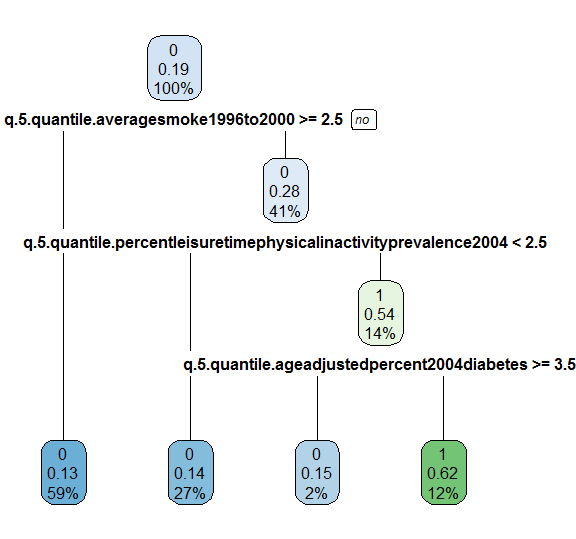
\includegraphics[width=3.25in]{decision-tree-01-paraclique-no-clustering.png}
\caption{Decision tree based on paraclique features, no clustering}
\label{decision.tree.01}
\end{figure}

% references section

% can use a bibliography generated by BibTeX as a .bbl file
% BibTeX documentation can be easily obtained at:
% http://mirror.ctan.org/biblio/bibtex/contrib/doc/
% The IEEEtran BibTeX style support page is at:
% http://www.michaelshell.org/tex/ieeetran/bibtex/
%\bibliographystyle{IEEEtran}
% argument is your BibTeX string definitions and bibliography database(s)
%\bibliography{IEEEabrv,../bib/paper}
%
% <OR> manually copy in the resultant .bbl file
% set second argument of \begin to the number of references
% (used to reserve space for the reference number labels box)

% JSS steps to compile latex + biblatex
% 1. pdflatex traffic-classification.tex
% 2. bibtex traffic-classification (will look for .aux extension, do not specify in argument though)
% 3. pdflatex traffic-classification.tex
% 4. pdflatex traffic-classification.tex (again)

\bibliographystyle{ieeetr}
\bibliography{datta}

\end{document}
